\documentclass{article}
\usepackage[utf8]{inputenc}
\usepackage{graphicx}
\usepackage[hidelinks,linktoc=none]{hyperref}

\title{Software Design Document}
\author{Viper-Rocks 3338}
\date{\today}

\begin{document}
\maketitle

\tableofcontents
\newpage

\section*{Version History}
\begin{tabular}{|l|l|p{8cm}|}
\hline
\textbf{Version} & \textbf{Date}       & \textbf{Description} \\\hline
1.0   & May 16, 2025          & Initial outline: core requirements and architecture \\\hline
2.0   & May 23, 2025          & Added reporting and CSV export features \\\hline
3.0   & May 30, 2025          & Snapshot 3: integrated TestRail, refined tech stack and UI frameworks \\\hline
4.0   & \today                & Snapshot 4: added workflow diagram and final polish \\\hline
\end{tabular}

\section{Introduction}
\begin{itemize}
  \item \textbf{Purpose:} Present the design blueprint for the Lunar Rocks! analysis tool, covering component interactions, data flows, and UI architecture
  \item \textbf{Intended Audience:} Development team, testers, and project stakeholders
  \item \textbf{Overview:} Snapshot 4 finalizes system design by adding a high-level workflow diagram and refining UI and architecture details
\end{itemize}

\section{System Architecture}
\begin{itemize}
  \item \textbf{Architecture Pattern:} Separation of front-end (React + Next.js) and back-end (Node.js REST API)
  \item \textbf{Tech Stack:} React 18, Next.js 14, Konva.js for canvas tasks; Node.js + Express; PostgreSQL 16 with PostGIS; Sequelize ORM; QGIS for preprocessing
  \item \textbf{Data Flow Diagrams:} Level 0 outlines user interactions; Level 1 details core modules and data pipelines
  \item \textbf{Services:} CSV export endpoint; reporting engine aggregates metrics; TestRail connector displays test-run summaries
\end{itemize}

\section{Workflow Diagram}
\begin{figure}[h]
  \centering
  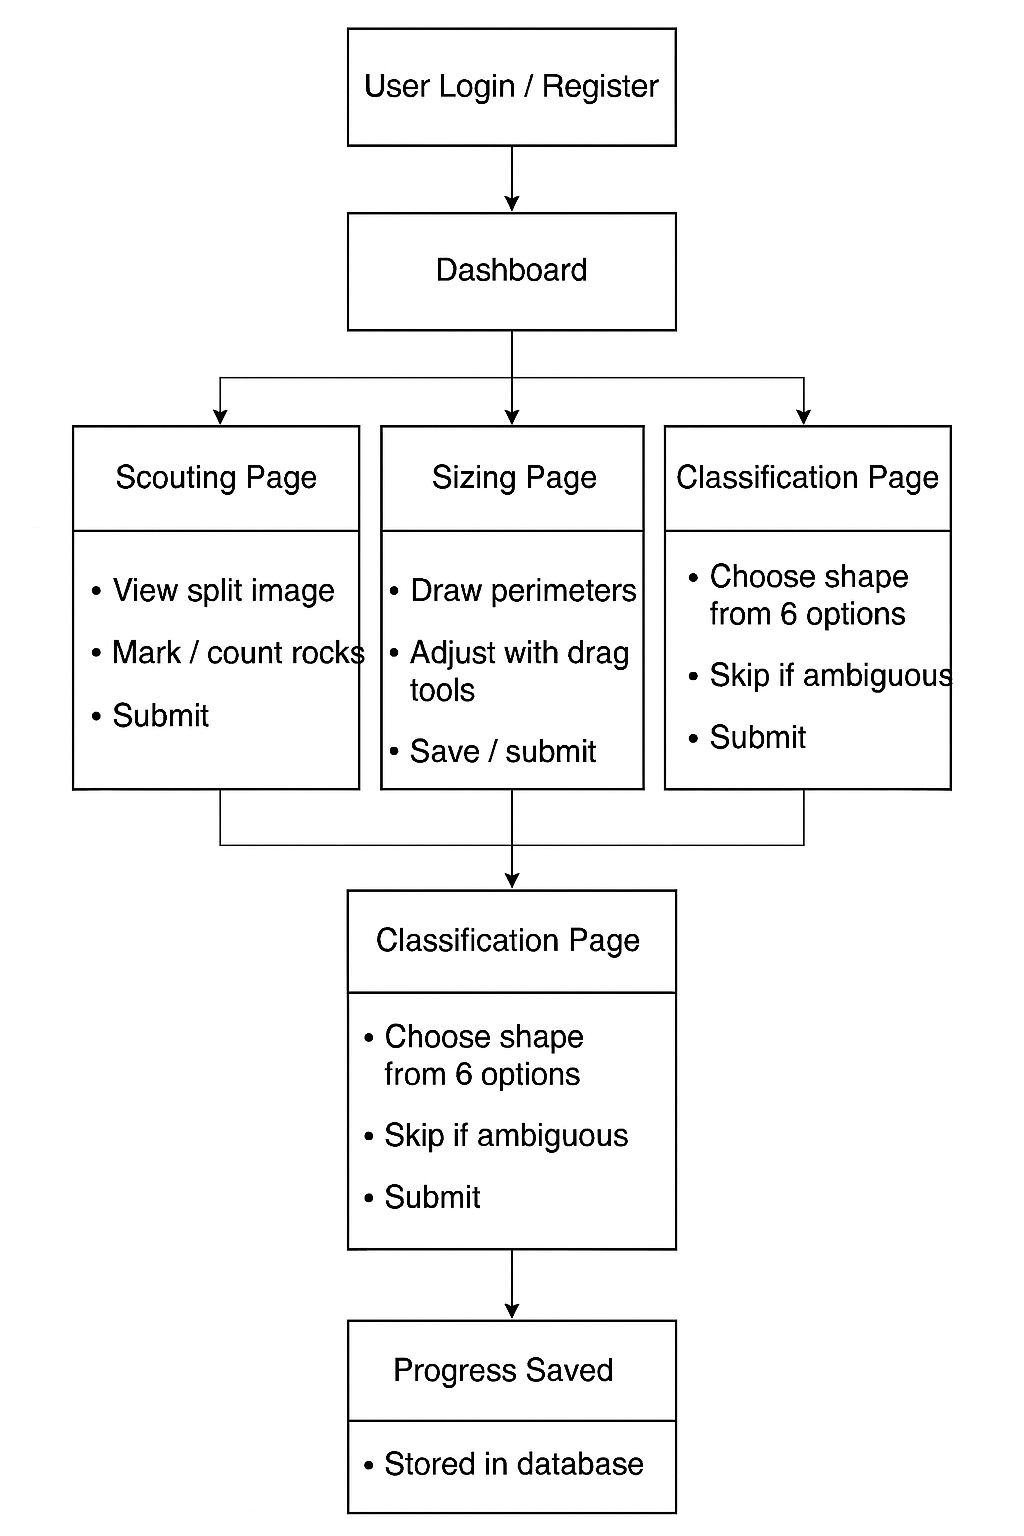
\includegraphics[width=0.9\textwidth]{images:Workflow_Diagram_Lunar_Rocks.png}
  \caption{High-level user workflow from login through scouting, sizing, classification, and data storage}
  \label{fig:workflow}
\end{figure}

\section{User Interface}
\subsection{UI Frameworks}
\begin{itemize}
  \item Based on JPL’s Explorer-1 Design System with React and TailwindCSS
  \item Accessibility focused keyboard navigation, screen-reader labels
  \item Simple clean interface with clearly labled features
\end{itemize}

\subsection{Primary Screens}
\begin{itemize}
  \item \emph{Upload}: File picker and project selector dashboard
  \item \emph{Scouting}: Auto-numbered segment gallery
  \item \emph{Sizing Canvas}: Konva-based measurement tools with undo/redo
  \item \emph{Classification}: Category icons with visual guidance
  \item \emph{Reporting Dashboard}: Filterable tables and charts
  \item \emph{Export Dialog}: CSV/PDF format chooser and download
  \item \emph{TestRail Dashboard}: Shows linked test runs and pass/fail statuses
\end{itemize}

\subsection{Database Integration}
\begin{itemize}
  \item Sequelize with connection pooling for time efficient queries
  \item Entities: users, images, segments, measurements, classifications, test_runs
\end{itemize}

\section{Glossary}
\begin{description}
  \item[UI] User Interface
  \item[API] Application Programming Interface
  \item[DFD] Data Flow Diagram
  \item[CSV] Comma-Separated Values
  \item[PDF] Portable Document Format
  \item[TR] TestRail
  \item[ORM] Object-Relational Mapping
  \item[WCAG] Web Content Accessibility Guidelines
\end{description}

\section{References}
\begin{itemize}
  \item Project brief: \url{https://ascent.cysun.org/project/project/view/227}
  \item SRS source: \url{https://github.com/ChrislIlIIlIIl/Viper-Rocks/blob/main/docs/SRS.tex}
\end{itemize}

\end{document}
